\begin{sloppypar} % помогает в кириллическом документе выровнять текст по краям
\newpage % Так добавляется  новая страница

% \section*{ВВЕДЕНИЕ}%так объявляется новая глава. * означает, что эта глава не попадает в оглавление и не имеет номера.
% \addcontentsline{toc}{section}{\hspace{1mm}ВВЕДЕНИЕ} % эта строчка нужна, чтобы такую главу в оглавление все таки добавить, но без номера. Такие госты, что поделать.
% введение я вообще снес нахуй, так как не придумал, что там писать.



\section{Часть I} %Объявили начало главы
\subsection{Создание проекта и описание устройства с помощью VHDL} %Объявили начало раздела
По методике, описанной в методических указаниях к лабораторной работе, в программном пакете Vivado v2016.4 был создан проект.


Для описания портов и логики схемы используется файл с описанием устройства на языке VHDL \textit{fdc.vhd}, содержимое которого можно увидеть ниже:

% код можно вставить с помощью команды прямо из файла

\inputminted[
% frame=lines,%линия сверху и снизу блока кода
% framesep=15mm, % отступ между линией и кодом
baselinestretch=1, %интервал междустрочный
% bgcolor=LightGray, %цвет фона
fontsize=\footnotesize, %размер шрифта
% linenos%нумерация строк
]
{VHDL}%язык программирования
{fdc.vhd}%файл с кодом(должен лежать в папке проекта)

Данный код описывает в одном модуле всю схему, представленную на
рисунке 1. Первый блок \textit{process (C)} описывает логику D-триггеров DD1 и
DD2. Второй блок \textit{process (C) }– логику конъюнктора DD3 и D-триггера DD4.

% код так же можно вставить вот так, прямо кодом, не через файл.
% \begin{minted} [
% frame=lines,%линия сверху и снизу блока кода
% framesep=15mm, % отступ между линией и кодом
% baselinestretch=1, %интервал междустрочный
% bgcolor=LightGray, %цвет фона
% fontsize=\footnotesize, %размер шрифта
% linenos%нумерация строк
% ]{VHDL}
% library IEEE;
% use IEEE.STD_LOGIC_1164.ALL;

% entity fdc is 
    % Port (D_0, D_1: in STD_LOGIC;
    % C : in STD_LOGIC;
    % Q : out STD_LOGIC);
% end fdc;

% architecture Behavioral of fdc is

% signal x_0, x_1 : STD_LogIC;
    
% begin
    % process (C)
    % begin
        % if rising_edge(C) then
        % X_0 <= D_0;
        % X_1 <= D_1;
    % end if;
% end process;
    % process (C)
    % begin
        % if rising_edge(C) then
        % Q<= X_0 and X_1;
        % end if;
    % end process;
% end Behavioral;
% \end{minted}

% С кодом разобрались, окей
\subsection{Симуляция устройства} %Объявили начало раздела

Следующий этап - симуляция устройства.
Для этого был создан файл симуляции (Test bench) tb\_sim.vhd на языке VHDL, содержимое которого можно увидеть ниже:
\inputminted[
% frame=lines,%линия сверху и снизу блока кода
% framesep=15mm, % отступ между линией и кодом
baselinestretch=1, %интервал междустрочный
% bgcolor=LightGray, %цвет фона
fontsize=\footnotesize, %размер шрифта
% linenos%нумерация строк
]
{VHDL}%язык программирования
{tb_sim.vhd}%файл с кодом(должен лежать в папке проекта)

После запуска симуляции были получены временные диаграммы, изображенные на рисунке \ref{ris:Figures/2022-10-10_22-59-24.png}.

\imgh{160.5mm}{Figures/2022-10-10_22-59-24.png}{Результат симуляции} %можно так вставить изображение
% так, с изображением разобрались, есть еще такой способ, с одной стороны чуть более гибкий, с другой - длиннее код

% \begin{figure}[!htb]
	% \centering
	% 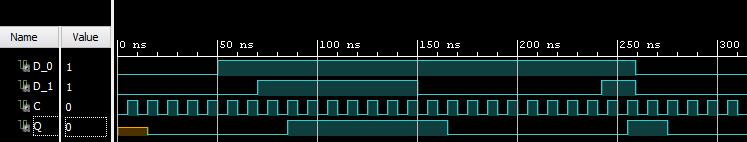
\includegraphics[width=\textwidth]{Figures/2022-10-10_22-59-24.png}
	% \caption{Здесь может быть указана подпись рисунка}\label{fig:Figures/2022-10-10_22-59-24.png}
% \end{figure}
% Параметр width задаёт ширину рисунка. В этом случае она равна ширине текста, \textwidth. Вместо \textwidth можно укзать значение от 0.1 до 1. \label нужен для того, чтобы потом можно делать сноску на эту картинку, как было выше(ну где  написано типа \ref{ris:Figures/2022-10-10_22-59-24.png}.)

\newpage % ебанем новую страницу
\subsection{Синтез цифрового устройства} %Объявили начало раздела
В этом этапе необходимо было провести тщательный временной анализ, необходимый для обнаружения узких мест и обеспечения эффективной и надежной работы устройства. 
В результате синтеза была получена следующая схема (рисунок \ref{ris:Figures/2022-10-11_19-48-02.png})

\imgh{160.5mm}{Figures/2022-10-11_19-48-02.png}{Синтезированная схема}
\imgh{160.5mm}{Figures/2022-10-11_20-10-59.png}{Принципиальная схема из методических указаний к лабораторной работе}

От принципиальной схемы, изображенной в методических указаниях в начале работы (рисунок \ref{ris:Figures/2022-10-11_20-10-59.png}), полученная в результате синтеза схема отличается наличием буферных каскадов IBUF и OBUF(вероятно, это сокращения от input и output buffer), по всей видимости необходимых для согласования по логическим уровням напряжения и согласования сопротивлений.. Так же отличием можно считать элемент BUFG, который нужен, как я понял, для того, чтобы использовать глобальный тактовый сигнал. Не совсем понял, как это реализовано в железе: это какая-то выделенная шина с тактовым сигналом внутри микросхемы?


\subsubsection{Временные ограничения} %Объявили начало подраздела
Тут по моему скромному мнению нужно дохуя почитать харриса или глянуть лекции, потому что я лично понимяо нихуя и только на пальцах

в результате все это говно надо связать с рисунком \ref{ris:Figures/2022-10-11_22-17-53.png}

\imgh{160.5mm}{Figures/2022-10-11_22-17-53.png}{хуевременные задержки}


\newpage
\subsection{РЕАЛИЗАЦИЯ} %Объявили начало раздела


Про автоматическую расстановку портов что то нахуй,или еще что. можно ебануть ту картинку с морским боем


\subsection{Индивидуальные задания}%такая глава попадает в оглавление и имеет номер.
1. Выясните, какая максимальная частота работы схемы возможна при заданных временных ограничениях.


2. Выберите ПЛИС с другими параметрами (опции -2 или -3 в названии) и определите, какая максимальная частота возможна для них.


3. Установите вручную положение вывода Clock на E3 и заставьте Vivado автоматически разместить все остальные выводы.


4. Вернитесь к этапу моделирования и повторите его используя «Run Post-Synthesis Functional Simulation», «Run Post-Synthesis Timing Simulation», «Run Post-Implementation Functional Simulation» и «Run Post-Implementation Functional Simulation». Сравните полученные результаты с результатами, полученными в разделе 2.


5. Повторите пункт 4, задав другую частоту тактового сигнала.


6. Добавьте к наблюдаемым сигналам внутренние сигналы (выходы элемента «И» и триггеров первой ступени) и посмотрите, как выполняются временные соотношения









\section*{ОТВЕТЫ НА ВОПРОСЫ ДЛЯ САМОПРОВЕРКИ}
\addcontentsline{toc}{section}{\hspace{1mm}ОТВЕТЫ НА ВОПРОСЫ ДЛЯ САМОПРОВЕРКИ}

1. Какие два подхода к описанию аппаратуры вы знаете? Какой подход
вы использовали в лабораторной работе?


2. Какие языки описания аппаратуры (HDL) вы знаете? Какой язык вы
использовали в лабораторной работе?


3. Какой программный пакет и какую ПЛИС вы использовали в лабораторной работе?


4. Опишите стандартный процесс проектирования цифровых устройств.


5. Вспомните таблицу переходов D-триггера и таблицу истинности логического вентиля И.


6. Для чего нужна симуляция устройства на поведенческом уровне?


7. Для чего необходимо задавать временные задержки?


8. На каком этапе проектирования цифровых устройств строится топология проекта и подключаются внешние выводы?


9. Опишите назначение строк кода в файле fdc.vhd.


10. Опишите назначение строк кода файла симуляции tb\_sim.vhd.


11. Нарисуйте временную диаграмму работы вашего устройства и сравните ее с диаграммой, полученной в результате симуляции.


12. Что такое ограничения проектирования и для чего они нужны?


13. Какие временные ограничения вы задавали в вашем проекте?




% \newpage
% \bibliographystyle{plain}
% \bibliography{bibliography}


\end{sloppypar}
